\subsection{M\'etodos computacionales}
\frame{
	\frametitle{M\'etodos computacionales}
	\begin{itemize}
		\item Se Utiliza el software Quantum-Espresso para realizar los c\'alculos de primeros principios.
		\pause
		\item Se utilizan dos computadoras que se encuentran equipadas con un procesador con 8 n\'ucleos y 32 GB de memoria RAM.
	\end{itemize}
}
\subsubsection{Materiales}
\frame{
	\frametitle{Materiales}
	\begin{columns}
		\column{0.4\textwidth}
		       \begin{figure}
		       	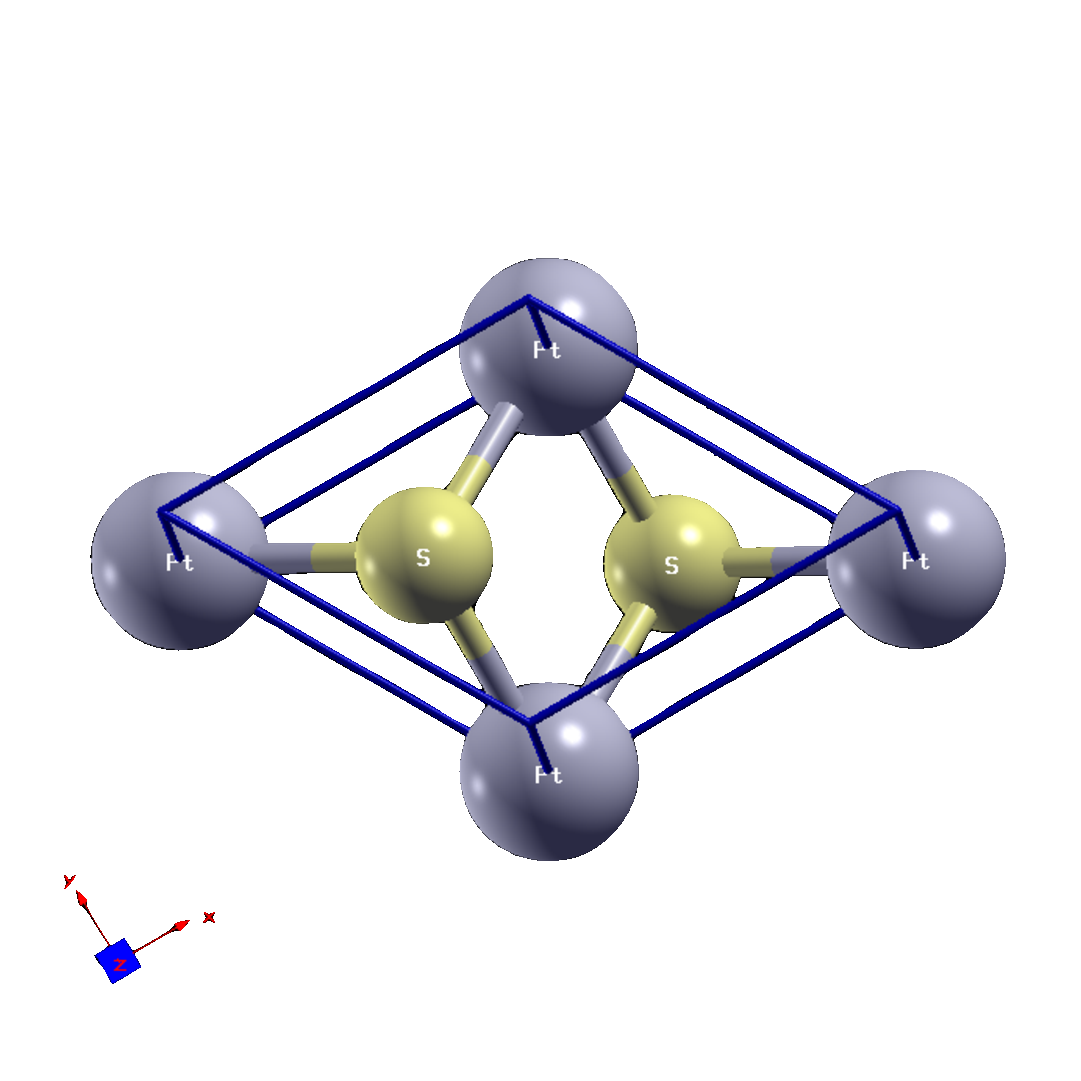
\epsfig{file=figMet/superceldaarriba.eps, width=5.0cm,height=5.0cm}
		       	\caption{Supercelda para c\'alculos sin defectos.}
		       \end{figure}
		    	
		%
		\column{0.6\textwidth}
		\begin{itemize}
			\item Estructura $1T$.
			\pause
			\item PtSe\textsubscript{2}, PtS\textsubscript{2}, VSe\textsubscript{2} y VS\textsubscript{2}
			\pause
			\item Modelos de materiales creados en VESTA a partir de estructuras disponibles en una base de datos en donde se le agrega una capa de vac\'io.
		\end{itemize}
	\end{columns}
}
\frame{
	\frametitle{Tabla peri\'odica}
	\begin{figure}[!hbt]
		\centering
		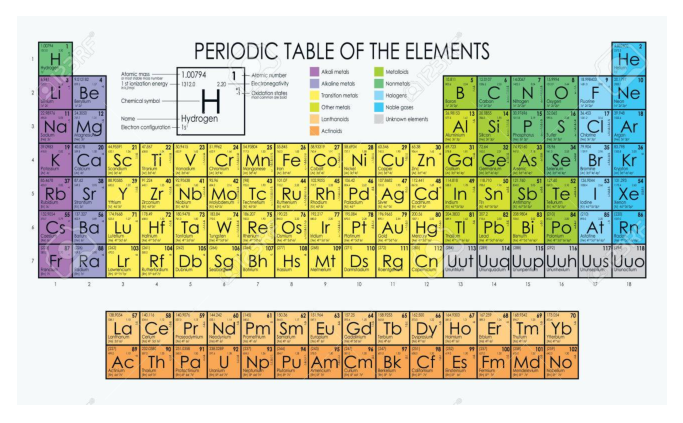
\epsfig{file=figRes/tabla-periodica-de-los-elementos.eps, scale=1}
	\end{figure}
	
}
\frame{
	\frametitle{Orbitales de los \'atomos utilizados}
	\begin{itemize}
		\item Metales de transici\'on:
		\pause
		\begin{itemize}
			\item Pt $\leftarrow~~5d^{9}~ 6s^{1}$
			\pause
			\item V $\leftarrow~~3d^{3}~4s^2$
		\end{itemize}
	    \pause
	    \item Calc\'ogenos:
	    \begin{itemize}
	    	\item S $\leftarrow~~3s^{2} ~3p^{4}$
	    	\pause
	    	\item Se $\leftarrow~~4s^{2} ~4p^{4}$
	    \end{itemize}
	\end{itemize}
}
\begin{frame}{Valores para la energ\'ia de corte y mapeo de Monkhorst y Pack}
	\begin{table}
		\caption[Valores de la energ\'ia de corte y mapeo de Monkhorst-Pack.]{Muestra los valores para la energ\'ia de corte y el mapeo en el espacio rec\'iproco (mapeo de Monkhorst y Pack) para las estructuras utilizadas en este trabajo.}
		\begin{tabular}{|c|c|m{5 cm}|} 
			\hline
			Material       &   $E_{corte}~~(Ry)$     & mapeo de Monkhorst y Pack $(k\times k \times 1)$  \\
			\hline
			\hline
			$PtS_2$        &   $60 $             &  $~~~~~~11 \times 11 \times 1$ \\
			$PtSe_2$        &   $63 $             &  $~~~~~~11 \times 11 \times 1$ \\
			$VS_2$        &   $80 $             &  $~~~~~~21 \times 21 \times 1$ \\
			$VSe_2$        &   $84 $             &  $~~~~~~21 \times 21 \times 1$ \\
			\hline
		\end{tabular}
	\end{table}
\end{frame}
\subsubsection{Creaci\'on del modelo de  la  vacancia de metal de transici\'on}
\frame{
	\frametitle{Creaci\'on del modelo de  la  vacancia de metal de transici\'on}
	\begin{columns}
		\column{0.4\textwidth}
		\begin{figure}
			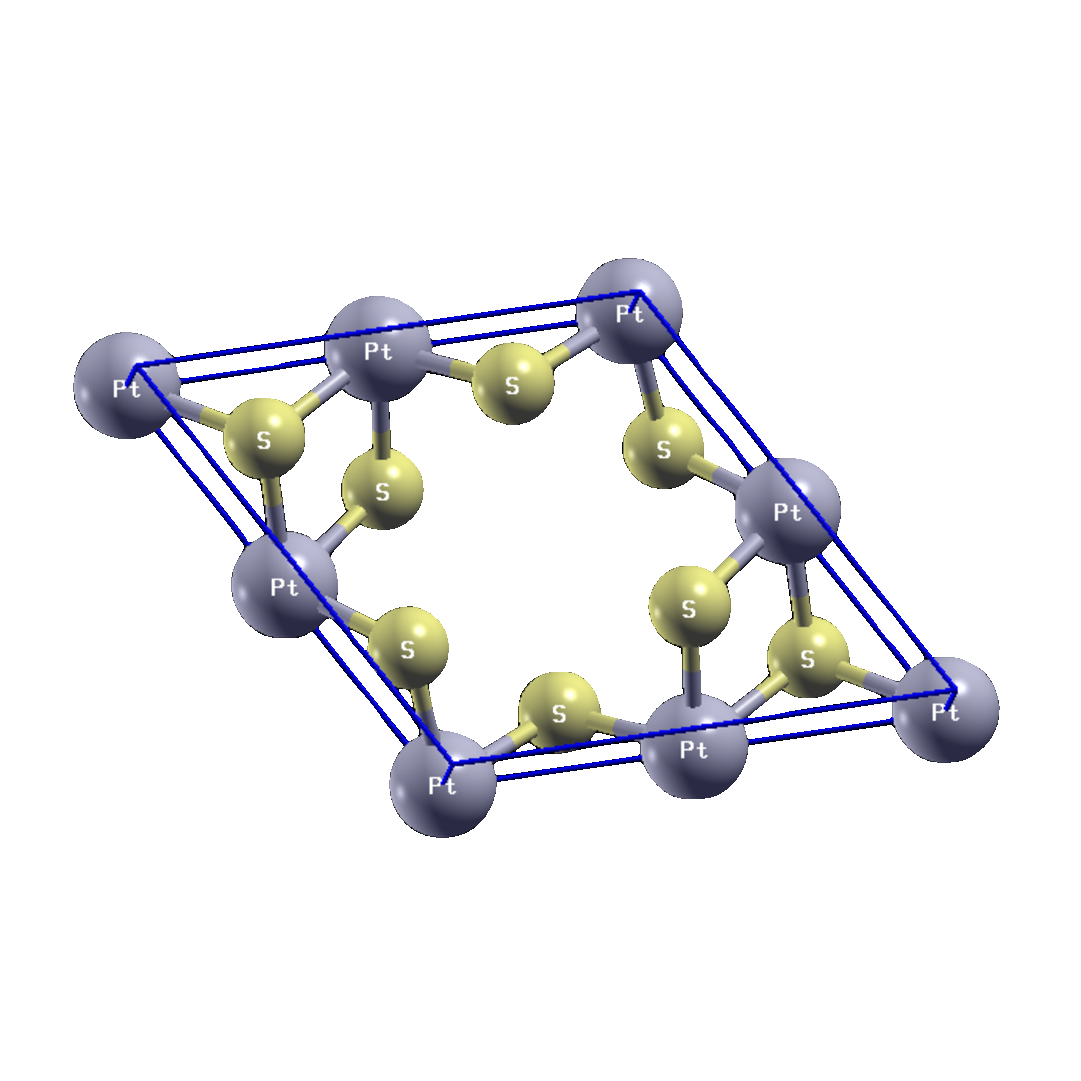
\epsfig{file=figMet/superceldaVacanciaArriba.eps, width=5.0cm,height=5.0cm}
			\caption{Supercelda para c\'alculos con vacancia del metal de transici\'on.}
		\end{figure}
			
		%
		\column{0.6\textwidth}
			\begin{itemize}
				\item Se crean con VESTA repitiendo dos veces la celda unitaria en las direcciones $a$ y $b$
				\pause
				\item Es necesario realizar una optimizaci\'on geom\'etrica.
			\end{itemize}
	\end{columns}
}	
\subsubsection{Deformaciones mec\'anicas}
\frame{
	\frametitle{Deformaciones mec\'anicas}
	\begin{figure}[hbt!]
		\centering
		\subfigure[]{
			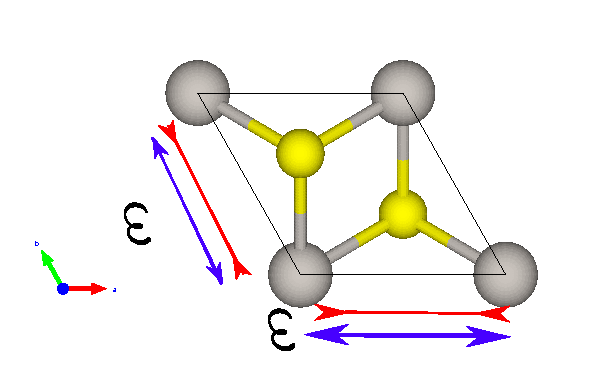
\epsfig{file=figMet/strainIso.eps, scale=0.5}
			\label{Met:fig:strainiso}
		}
		\subfigure[]{
			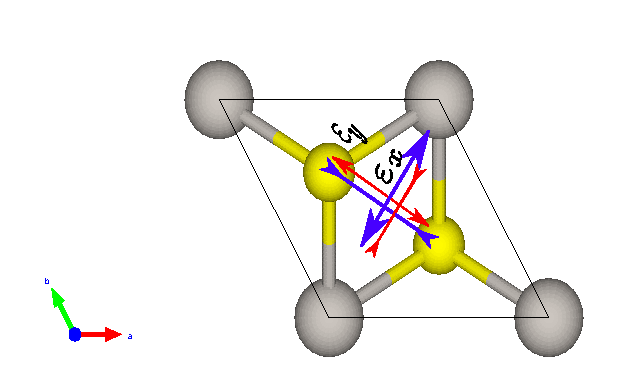
\epsfig{file=figMet/strainIAnis.eps, scale=0.5}
			\label{Met:fig:strainanis}
		}	
		\caption[Deformaciones estudiadas.]{Deformaciones estudiadas en este trabajo. \ref{Met:fig:strainiso} Muestra la aplicaci\'on de una deformaci\'on isotr\'opica en direcci\'on de los ejes cristalinos y \ref{Met:fig:strainanis} una deformaci\'on dirigida en la direcci\'on de los ejes cartesianos.}
	\end{figure}
}
\frame{
	\begin{itemize}
		\item Para el c\'alculo de la deformaci\'on se utiliza la siguiente expresi\'on:
		\begin{equation}
			\varepsilon = \frac{a-a_0}{a_0}. \label{Met:ec:strain}
		\end{equation}
	\pause
	\item Despu\'es de aplicar esta deformaci\'on es necesario realizar una optimizaci\'on geom\'etrica para que los \'atomos se coloquen en su nueva posici\'on de equilibrio.
	\end{itemize}
}
\begin{comment}


\subsubsection{C\'alculos realizados con Quantum Espresso}
\frame{
	\frametitle{C\'alculos realizados con Quantum Espresso}
	\begin{itemize}
		\item Evaluaci\'on auto consistente por medio del programa pw.x para encontrar la energ\'ia total del sistema, para realizar la optimizaci\'on geom\'etrica y el c\'alculo de la magnetizaci\'on.
		\pause
		\item Se utiliza pw.x para realizar un c\'alculo no auto consistente necesario para obtener el diagrama de bandas y la densidad de estados.
		\pause
		\item El programa band.x se usa para el c\'alculo del diagrama de bandas, dos.x para el c\'alculo de la densidad de estados y projdos.x para obtener la densidad de estados proyectada en los orbitales at\'omicos.
	\end{itemize}
}
\end{comment}
\frame{
	\frametitle{Par\'ametros de los c\'alculos auto consistentes}
	\begin{itemize}
		\item Se utiliza la aproximaci\'on de PBE \nocite{PhysRevLett.77.3865} para la funcional $E_{XC}$.
		\pause
		\item Se emplea el pseudo potencial  PAW  \nocite{PhysRevB.59.1758, PhysRevB.50.17953}con correcciones relativistas (para c\'alculos de magnetizaci\'on no colineal) y sin estas (para el caso colineal).
		\pause 
		\item Para el c\'alculo de optimizaci\'on geom\'etrica se utiliza el algoritmo BFGS.
	\end{itemize}
}
\frame{
	\frametitle{Puntos en la primera zona de Brillouin}
	\begin{columns}
		\column{0.4\textwidth}
            \begin{figure}
            	%\centering
            	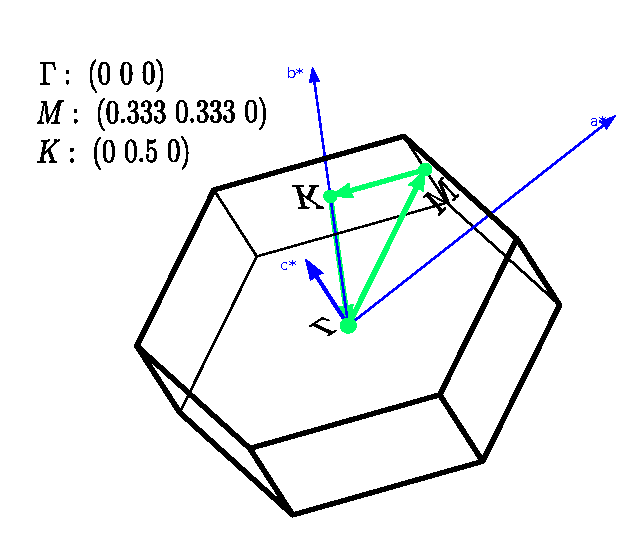
\epsfig{file=figMet/espacioK2.eps, width=5.0cm,height=5.0cm }
            	\caption{Primera zona de Brillouin con sus puntos especiales.}
            \end{figure}
				

	   %
	   \pause
	   \column{0.6\textwidth}
	   		\begin{itemize}
	   			\item $K-\Gamma-M-K$ para el PtSe\textsubscript{2} y PtS\textsubscript{2}
	   			\pause
	   			\vspace{0.7cm}
	   			\item $\Gamma-M-K-\Gamma$ para el VSe\textsubscript{2} y VS\textsubscript{2}
	   		\end{itemize}
	\end{columns}
}
\endinput
